% !TeX root = ../main.tex

\section{Kotlin Multiplatform Mobile}
\parindent=0pt
Kotlin Multiplatform Mobile\footnote{\url{https://kotlinlang.org/lp/mobile/}} (KMM) è un framework per lo sviluppo di app iOS e Android basato sul concetto di condivisione della logica applicativa mantenendo lo sviluppo nativo della UX/UI\footnote{User Experience/User Interface}. Consiste in un caso d'uso specifico (e il più diffuso) del framework Kotlin MultiPlatform (KMP), il quale permette di sviluppare il codice in modo agnostico rispetto le piattaforme target e di condividerlo tra differenti piattaforme facendo uso dei tre principali compilatori inclusi nell'ecosistema Kotlin\cite{nagy2022simplifying}:
\begin{itemize}
    \item Kotlin/JVM (Android, Spring, ...)
    \item Kotlin/Native (iOS, macOS, ...)
    \item Kotlin/JS (Web)
\end{itemize}
KMM dipende fortemente dai compilatori Kotlin/JVM (Android) e Kotlin/Native (iOS) e fornisce benefici derivanti sia dallo sviluppo cross-platform che dallo sviluppo nativo:
\begin{itemize}
    \item risparmio di tempo e risorse derivanti dalla condivisione del codice (cross-platform),
    \item alte performance (nativo),
    \item accesso diretto alle funzionalità dei dispositivi hardware senza overhead (nativo).
\end{itemize}

\begin{figure}[H]
\centering
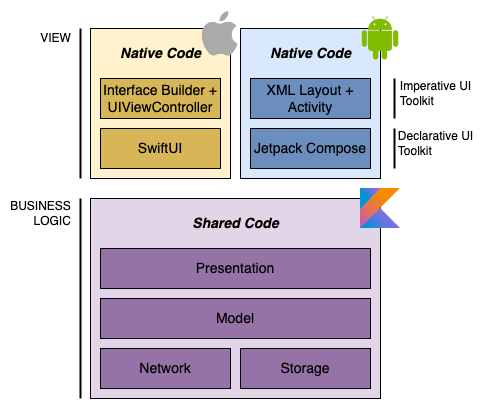
\includegraphics[width=0.7\textwidth]{img/tesi-8-kmm.drawio.png}
\caption{Architettura Kotlin Multiplatform Mobile}
\end{figure}

Con il rilascio di Kotlin 1.4 (Agosto 2020), KMM è passato dalla fase "\textit{Experimental}" alla fase "\textit{Alpha}" la quale è considerata come fase "\textit{pre-stable}"\footnote{\url{https://kotlinlang.org/docs/components-stability.html\#stability-levels-explained}} ma è comunque già stato adottato in produzione per lo sviluppo delle proprie applicazioni mobile da tantissime aziende tra le quali è possibile trovare nomi rilevanti come Netflix, VMware e Philips\footnote{\url{https://kotlinlang.org/lp/mobile/case-studies/}}.\\
In base al risultato dell'indagine di mercato svolta nei primi due quadrimestri del 2021\cite{kmm2}, le porzioni di codice condiviso nelle applicazioni sviluppate con KMM sono:
\begin{itemize}
    \item 85\% Networking
    \item 75\% Data Storage
    \item 70\% Utility (Logging, Analytics, ...)
    \item $\sim$60\% Algoritmi/Computazione
    \item $\sim$55\% State Management
    \item $\sim$50\% Presenters/Controllers/ViewModel
\end{itemize}

\subsection{Kotlin/JVM}
Il compilatore Kotlin/JVM è uno dei due compilatori su cui è basato KMM, utilizzato per la piattaforma Android. Permette di compilare codice Kotlin in bytecode Java (\textit{.class}), il quale può essere eseguito direttamente sulla JVM. Nel caso di Android è necessario un ulteriore passaggio per tradurre il bytecode Java in bytecode Dalvik (\textit{.dex}).

\begin{figure}[H]
\centering
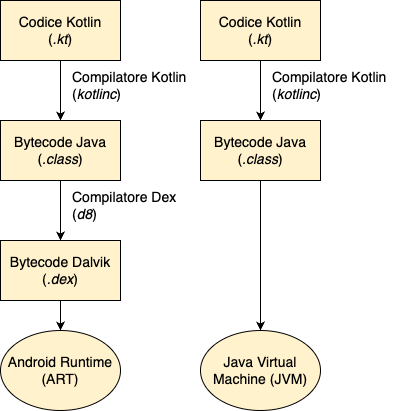
\includegraphics[width=0.55\textwidth]{img/tesi-9-kotlinjvm.drawio.png}
\caption{Fasi di compilazione Kotlin/JVM con piattaforma target Android e JVM}
\end{figure}

\subsection{Kotlin/Native}
Kotlin/Native è il secondo compilatore su cui è basato KMM e viene utilizzato per la piattaforma iOS. A differenza del compilatore Kotlin/JVM, il compilatore Kotlin/Native è progettato per quelle situazioni dove non è possibile o non si vuole avere una VM come nel caso dei dispositivi embedded e della piattaforma iOS. Per fare ciò include un backend basato su \textit{Low Level Virtual Machine} (LLVM)\footnote{\url{https://llvm.org/}}, ovvero il codice Kotlin viene compilato in binari nativi che possono essere eseguiti senza VM\cite{nagy2022simplifying}. Le piattaforme supportate da Kotlin/Native attualmente sono macOS, iOS, tvOS, watchOS, Linux, Windows (MinGW) e Android NDK\footnote{\url{https://kotlinlang.org/docs/native-overview.html\#target-platforms}} e per ognuna di esse esistono differenti architetture. Nel caso di iOS le differenti architetture supportate da KMM sono \textit{Arm64}, \textit{Arm32} e \textit{x64}.
\begin{figure}[H]
\centering
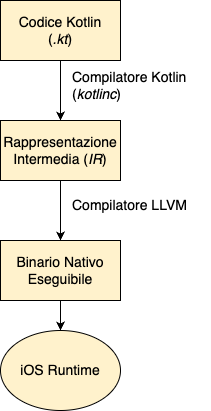
\includegraphics[width=0.28\textwidth]{img/tesi-10-kotlinnative.drawio.png}
\caption{Fasi di compilazione Kotlin/Native con piattaforma target iOS}
\end{figure}
Anche in questo caso sono necessarie due fasi di compilazione: ($i$) il codice Kotlin viene compilato nella \textit{Rappresentazione Intermedia} (IR) LLVM e ($ii$) successivamente compilato nel binario nativo.

\subsection{Expect/Actual}
Quando si sviluppa codice condiviso è spesso necessario definire come determinate funzionalità debbano essere implementate sulla specifica piattaforma target per utilizzare i relativi SDK. Il framework KMP fornisce il meccanismo \textit{expect/actual} per assolvere a questo compito in modo analogo al design pattern \textit{Template Method}:
\begin{itemize}
    \item \textit{Expect} - Astrazione della funzionalità necessaria. Tramite la keywork \textit{expect} si definisce lo scheletro astraendo dalla specifica implementazione.
    \item \textit{Actual} - Implementazione specifica per una determinata piattaforma. Tramite la keywork \textit{actual} si definisce l'implementazione, reificando l'altrazione definita tramite il concetto di \textit{expect}.
\end{itemize}

\begin{listing}[H]
\inputminted{kotlin}{code/3-expectactual}
\caption{Esempio di applicazione expect/actual per ottenere informazioni sulla piattaforma}
\end{listing}

\subsection{Plugin Gradle KMP}
Il plugin Gradle KMP è uno strumento utile per realizzare progetti multiplatform. Fornisce uno specifico DSL\footnote{Domain Specific Language} per definire e configurare i task necessari a compilare il codice condiviso per le relative piattaforme target\footnote{\url{https://kotlinlang.org/docs/multiplatform-dsl-reference.html}}. Al momento la versione latest (stable) del plugin è la \textit{1.6.21}, rilasciata il 19/04/2022\footnote{\url{https://plugins.gradle.org/plugin/org.jetbrains.kotlin.multiplatform/1.6.21}} ma è presente una versione candidata per il rilascio con tag \textit{1.7.0-RC2}.

\begin{listing}[H]
\inputminted{kotlin}{code/3-gradlekmm1}
\caption{Struttura iniziale del file \textit{settings.gradle.kts} nella root di progetto (Kotlin)}
\end{listing}

\begin{listing}[H]
\inputminted{kotlin}{code/3-gradlekmm2}
\caption{Definizione utilizzo Plugin Gradle KMP nel file \textit{build.gradle.kts} del modulo condiviso (Kotlin)}
\end{listing}

\subsubsection{Plugin Tasks}
Il plugin gradle KMM e le relative dipendenze rendono disponibile una vasta serie di task per eseguire differenti elaborazioni sia sul codice della specifica piattaforma target che sul codice condiviso. Alcune delle principali tipologie di task sono:
\begin{itemize}
    \item Build - tasks per build, compile, link
    \item CocoaPods - tasks per la gestione delle dipendenze Swift/Objective-C
    \item Interop - tasks relativi all'utilizzo del \textit{commonizer}\footnote{\url{https://github.com/JetBrains/kotlin/tree/master/native/commonizer}}
    \item Verification tasks - tasks per l'esecuzione dei test
\end{itemize}

\subsubsection{KMM Android Studio IDE Plugin}
L'IDE\footnote{Integrated Development Environment} Android Studio è costruito su IntelliJ, il quale è uno tra gli IDE più diffusi ed è sviluppato da JetBrains. Tramite il plugin KMM, installabile direttamente dal marketplace integrato in Android Studio o dal sito ufficiale JetBrains\footnote{\url{https://plugins.jetbrains.com/plugin/14936-kotlin-multiplatform-mobile/versions/stable}}, si abilita un insieme di funzionalità a supporto dello sviluppo di codice multiplatform, in particolare:
\begin{itemize}
    \item creazione della struttura e della configurazione base per una nuova applicazione multiplatform,
    \item creazione della struttura e della configurazione base per una nuova libreria multiplatform,
    \item integrazione di moduli multiplatform in applicazioni già esistenti.
\end{itemize}

\section{Fastlane}
Uno fra i tool open source più diffusi a supporto della automazione dello sviluppo di applicazioni mobile, sia Android che iOS, è Fastlane\footnote{\url{https://github.com/fastlane/fastlane}}. L'impiego principale di questo tool sviluppato in Ruby consiste nella automazione della fase di rilascio della applicazione, sia in beta che in produzione, grazie alla gestione di tutti quei task necessari ma dispendiosi in termini di tempo come ad esempio la generazione degli screenshot e la firma digitale del codice (\textit{Code Signing}).\\
Si fa uso dei seguenti concetti per controllare il comportamento di fastlane negli appositi file di configurazione \textit{Fastfile} e \textit{Appfile}:
\begin{itemize}
    \item \textit{Action} - Elaborazioni pre-definite e configurabili tramite passaggio di parametri.
    \item \textit{Lane} - Insieme di action definito dall'utente per descrivere elaborazioni complesse.
\end{itemize}

\begin{listing}[H]
\inputminted{ruby}{code/4-fastlane}
\caption{Esempio di definizione di un lane per il rilascio in versione beta di applicazioni iOS}
\end{listing}

I file \textit{Fastfile} e \textit{Appfile}, i quali risiedono nella cartella \textit{fastlane} nella root di progetto, sono utilizzati rispettivamente per definire configurazioni globali a livello di applicazione e per definire il comportamento di fastlane. Per questo motivo è necessario configurare fastlane per ogni modulo che si intende utilizzare, sia che esso sia una libreria o una applicazione. Nel caso di applicazioni multiplatform è quindi necessario per tutti i tre moduli \textit{shared}, \textit{androidApp} e \textit{iosApp}.\\
Nelle successive descrizioni delle fasi che compongono la pipeline progettata viene indicato come è stato configurato e adottato Fastlane ove utilizzato. 